\documentclass[10pt]{article}
\usepackage[total={170mm,230mm}]{geometry}

\usepackage{cmap}
\usepackage{hyperref}
\usepackage[utf8]{inputenc}
\usepackage[T2A]{fontenc}
\usepackage[russian]{babel}

\usepackage{graphicx}
\usepackage{xcolor}
\usepackage{amssymb}
\usepackage{amsfonts}
\usepackage{amsmath}
\usepackage{amsthm}
\usepackage{physics}
\usepackage{wrapfig}
\usepackage{cancel}
\usepackage{pdfpages}
\usepackage{hyperref}
% \usepackage{bibtex}

\title{Домашнее задание №3}
\author{Александр Козлов}
\date{\today}

\begin{document}

\maketitle

\section*{Формулировка задания}

Дан гамильтониан одномерной квантово-механической системы с потенциалом в виде гауссовой ямы
\begin{equation}
    H = - \dv[2]{}{x} + V_0\, e^{-x^2},
\end{equation}
где $V_0 < 0$. Требуется вычислить основное состояние с помощью метода простых итераций со сдвигом при значении постоянной связи $V_0$, которое поддерживает два состояния дискретного спектра. Исследовать зависимость вычислительных затрат от числа точек сетки.

\section{Численное решение}

Рассматриваемое уравнение Шрёдингера (УШ) имеет вид
\begin{equation}
    -\dv[2]{\psi}{x} + V_0\, e^{-x^2}\, \psi  = E\, \psi
    \label{eq:SE}
\end{equation}
или
\begin{equation}
    \dv[2]{\psi}{x}  + (E - V_0\, e^{-x^2})\, \psi  = 0.
\end{equation}
Стоит заметить, что такое уравнение соответствует обычному одномерному УШ при $\hbar=1$ и $m=1/2$.

Прежде всего зададим равномерную сетку
\begin{equation}
    x_0 = -R,\; x_1 = x_0 + \delta,\; x_2 = x_0 + 2\delta,\; \ldots,\; x_k = x_0 + k\delta,\; \ldots,\; x_M = x_0 + M \delta = R
\end{equation}
с шагом $\delta = 2R/M$, где $M$~---~целое положительное число, а $R$~---~положительное действительное число. Будем пользоваться численной аппроксимацией второй производной
\begin{equation}
    \dv[2]{\psi}{x}(x_k) = \dfrac{\psi(x_{k+1}) - 2\psi(x_{k}) + \psi(x_{k-1})}{\delta^2} + O(\delta^2),\quad k = \overline{1,M-1}
\end{equation}
и сводить уравнение \eqref{eq:SE} к задаче диагонализации трёхдиагональной матрицы.

Перед тем, как писать явный вид такой матрицы, необходимо поговорить о том, как будут задаваться граничные условия. Ясно, что волновые функции состояний дискретного спектра будут экспоненциально затухать при больших по абсолютному значению $x$. Это обстоятельство может быть численно учтено различными вариантами, однако, остановимся на варианте, при котором полагается $\psi(x_0) = \psi(x_M) = 0$. Тогда численное приближение УШ для $k=1$ примет вид
\begin{equation}
    -\dfrac{\psi(x_{2}) - 2\psi(x_{1})}{\delta^2} + V(x_1)\,\psi(x_1) = E\psi(x_1).
\end{equation}
Для $k=M-1$ получаем аналогичное уравнение
\begin{equation}
    -\dfrac{-2\psi(x_{M-1})+\psi(x_{M-2}) }{\delta^2} + V(x_{M-1})\,\psi(x_{M-1}) = E\psi(x_{M-1}).
\end{equation}
А для всех остальных $k$ имеем уравнение
\begin{equation}
    -\dfrac{\psi(x_{k+1}) - 2\psi(x_{k}) + \psi(x_{k-1})}{\delta^2} + V(x_k)\,\psi(x_k) = E\psi(x_k).
\end{equation}
В матричном виде задача записывается так:
\begin{equation}
\begin{split}
    &\begin{pmatrix}
        2\delta^{-2}+V(x_1)& -\delta^{-2}\\
        -\delta^{-2}& 2\delta^{-2}+V(x_2)& -\delta^{-2}\\
        % & -\delta^{-2}& 2\delta^{-2}+V_0\,e^{-x_3^2}& -\delta^{-2}\\
        & & & \ddots&\\
        & & & & -\delta^{-2}& 2\delta^{-2}+V(x_{M-2})& -\delta^{-2}\\
        & & & & & -\delta^{-2}& 2\delta^{-2}+V(x_{M-1})
    \end{pmatrix}
    \begin{pmatrix}
        \psi(x_1)\\
        \psi(x_2)\\
        \vdots\\
        \psi(x_{M-2})\\
        \psi(x_{M-1})
    \end{pmatrix}\\
    &=E
    \begin{pmatrix}
        \psi(x_1)\\
        \psi(x_2)\\
        \vdots\\
        \psi(x_{M-2})\\
        \psi(x_{M-1})
    \end{pmatrix}.
\end{split}
\end{equation}
Таким образом надо диагонализовать симметричную трёхдиагональную матрицу размера $(M-1)\times(M-1)$.

Но мы вместо того, чтобы диагонализовывать матрицу
\begin{equation}
 \hat H = \begin{pmatrix}
        2\delta^{-2}+V(x_1)& -\delta^{-2}\\
        -\delta^{-2}& 2\delta^{-2}+V(x_2)& -\delta^{-2}\\
        % & -\delta^{-2}& 2\delta^{-2}+V_0\,e^{-x_3^2}& -\delta^{-2}\\
        & & & \ddots&\\
        & & & & -\delta^{-2}& 2\delta^{-2}+V(x_{M-2})& -\delta^{-2}\\
        & & & & & -\delta^{-2}& 2\delta^{-2}+V(x_{M-1})
    \end{pmatrix},
\end{equation}
будем решать задачу более сложным путём~---~методом последовательных итераций со сдвигом. Для этого, сперва найдём методом простых итераций наибольшое по абсолютному значению собственное значение матрицы $\hat H$ $E_\textrm{max}$. Затем сдвинем спектр матрицы $\hat H$ на $E_\textrm{max}/2$, то есть перейдём к рассмотрению матрицы $\hat H_* = \hat H - E_\textrm{max}/2\; \hat I$. Найдём методом простых итераций наибольшее по модулю собственное значение новой матрицы.

\section{Результаты}

Метод простых итераций со сдвигом был применён для определения энергии основного состояния при фиксированных параметрах $R=6.0,\; V_0 = -5.0$ и при числе итераций, равном 1000, число точек сетки $M$ менялось, что дало зависимость времени вычисления от числа точек сетки, изображённую на Рис. \ref{fig:t_vs_m}.
\begin{figure}[htbp]
 \centering
 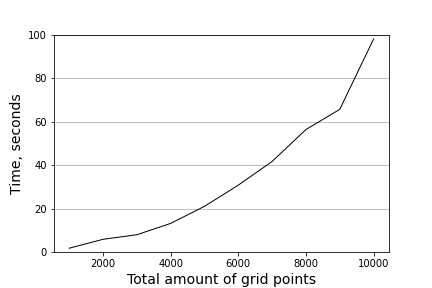
\includegraphics[width=0.75\textwidth]{../figures/t_vs_m}
 \caption{Зависимость времени работы программы в секундах от числа точек сетки при фиксированных $R=6.0,\; V_0 = -5.0$ и при 1000 итераций.}
 \label{fig:t_vs_m}
\end{figure}

Кроме того, удалось установить, что увеличение числа точек сетки при неизменной ширине сетки $R$ негативно сказывается на точности решения, что видно на Рис. \ref{fig:e1_vs_m}.
\begin{figure}[htbp]
 \centering
 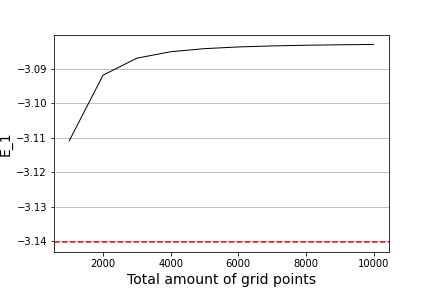
\includegraphics[width=0.75\textwidth]{../figures/e1_vs_m}
 \caption{Зависимость энергии основно состояния от числа точек сетки при фиксированных $R=6.0,\; V_0 = -5.0$ и при 1000 итераций. Чёрной линией отмечена полученная зависимость, красным пунктиром показано эталонное значение энергии основного состояния, взятое из первого домашнего задания.}
 \label{fig:e1_vs_m}
\end{figure}
У этого есть две основные причины. Во-первых, погрешность увеличивается применением такой операции, как вычисление разности двух больших чисел, которую применяем при переходе от максимального по модулю собственного значения матрицы $\hat H_* = \hat H - E_\textrm{max}/2\; \hat I$ к значения энергии основного состояния исходного гамильтониана $\hat H$. Во-вторых, при увеличении числа точек сетки неизменно уменьшается шаг сетки $\delta = 2R/M$, следовательно, увеличивается значение максимально большого значения энергии, которое мы можем оценить как $$E_\textrm{max} \sim 1/\delta^2\propto M^2$$ (напомним, что при постановке нулевых граничных условий гамильтониан фактически переходит к гамильтониану с бесконечными стенками, сильно возбужденные состояния которого будут зависеть от номера состояния пропорционально $n^2$), это приводит к чудовещному падению скорости сходимости. Поясним почему. Метод простых итераций со сдвигом  даёт оценку на точность получяемого в результате $k$ итераций значения максмальной по модулю энергии, как
\begin{equation}
 O\qty(\qty(\dfrac{E_{n-1}}{E_{n}})^{k+1}).
\end{equation}
Отсюда следует, что для матрицы со сдвинутыми собственными значениями оценка точности будет иметь вид
\begin{equation}
 O \qty( \qty(\dfrac{E_0 - E_\textrm{max}/2}{E_\textrm{max}/2})^{k+1} ) = O \qty( \qty(1-\dfrac{1}{M^2})^{k+1} ).
\end{equation}
Видно, что при увеличении $M$ точность падает.

\subsection{Более детальное доказательство того, что метод плох}
Из Рис. \ref{fig:e1_vs_m} может показаться, что с увеличением числа точек сетки результат куда-то сходится. Покажем, что это в корне не верно. Для этого введём в рассмотрение невязку
$$
R = \norm{\hat H \varphi_k - E_k \varphi_k},
$$
где $E_k$ и $\varphi_k$ --- полученное за $k$ итераций значение энергии и соответствующий ему собственные вектор. На Рис. \ref{fig:r_vs_m} показана зависимость такой невязки от числа точек сетки. Видно, что при малом числе точек сетки, алгоритм работает очень даже хорошо, но с увеличением числа точек сетки происходит стремительный рост невязки.
\begin{figure}[htbp]
 \centering
 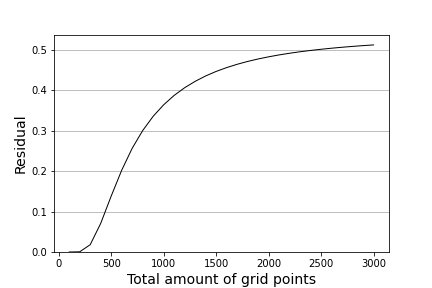
\includegraphics[width=0.75\textwidth]{../figures/r_vs_m}
 \caption{Зависимость невязки $R = \norm{\hat H \varphi_k - E_k \varphi_k}$ от числа точек сетки при фиксированных $R=6.0,\; V_0 = -5.0$ и при 1000 итераций.}
 \label{fig:r_vs_m}
\end{figure}



\end{document}
